\begin{figure*}[h!]
	\begin{subfigure}{\linewidth}
		\caption{}
		\centering
		% include first image
		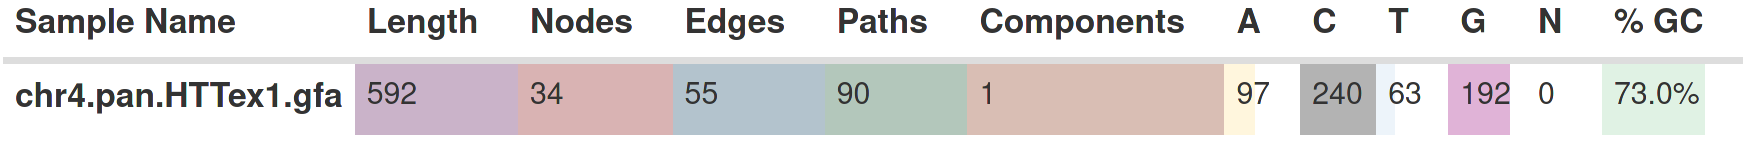
\includegraphics[width=1.0\linewidth]{fig/metrics/chr4_pan_HTTex1_gfa_multiqc_odgi_stats.png}  
		\label{fig:metrics-multiqc}
	\end{subfigure}
	\begin{subfigure}{\linewidth}
		\caption{}
		\centering
		% include second image
		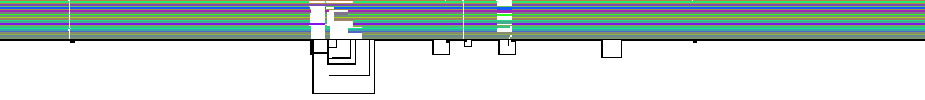
\includegraphics[width=1.0\linewidth, trim=0 0 -1cm 0 ]{fig/metrics/chr4_pan_fa_a2fb268_e820cd3_9ea71d8_smooth_gfa_og_HTTex1_og_O_og_tiny_og_png_svg.pdf}  
		\label{fig:metrics-viz}
	\end{subfigure}
	\begin{subfigure}{\linewidth}
		\caption{}
		\centering
		% include second image
		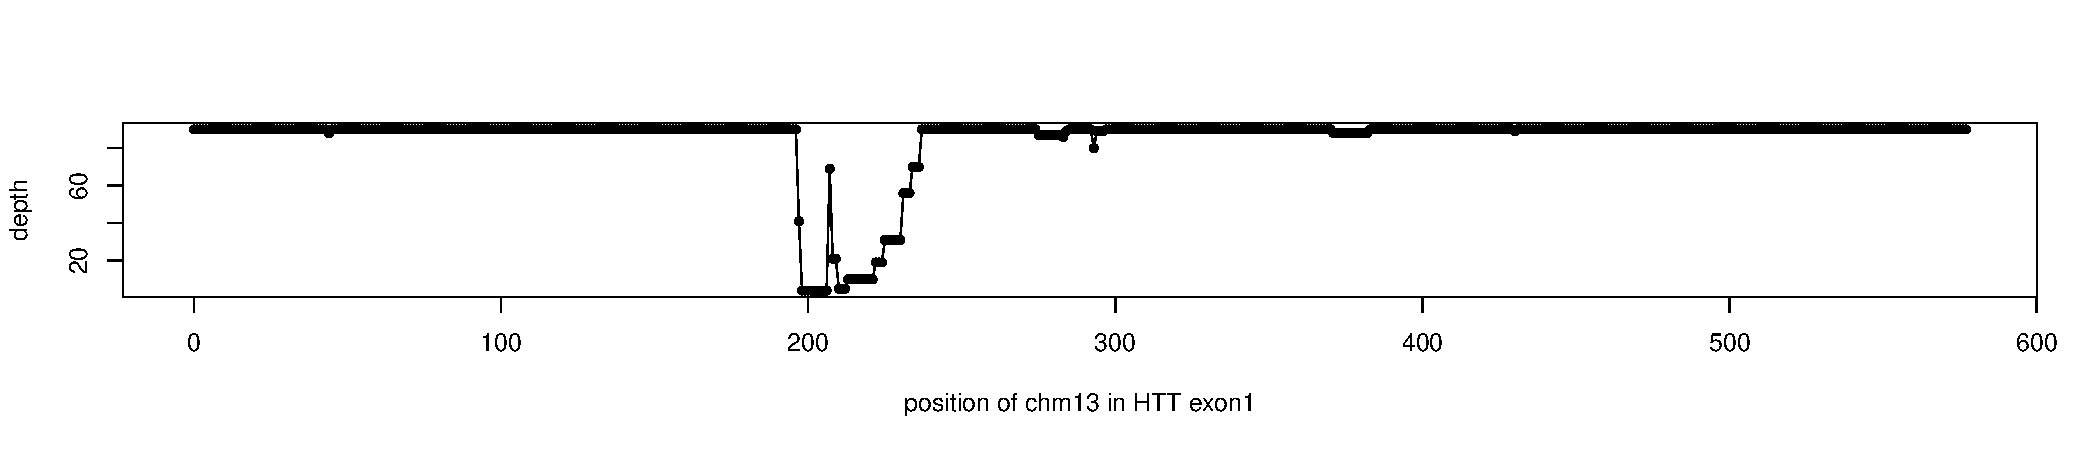
\includegraphics[width=\linewidth,trim=+.225cm 0 +0.425cm +2cm]{fig/metrics/chr4_HTT_chm13_depth_w1_bed.pdf}  
		\label{fig:metrics-depth}
	\end{subfigure}
	\begin{subfigure}{1\linewidth}
		\caption{}
		\centering
		% include fourth image
		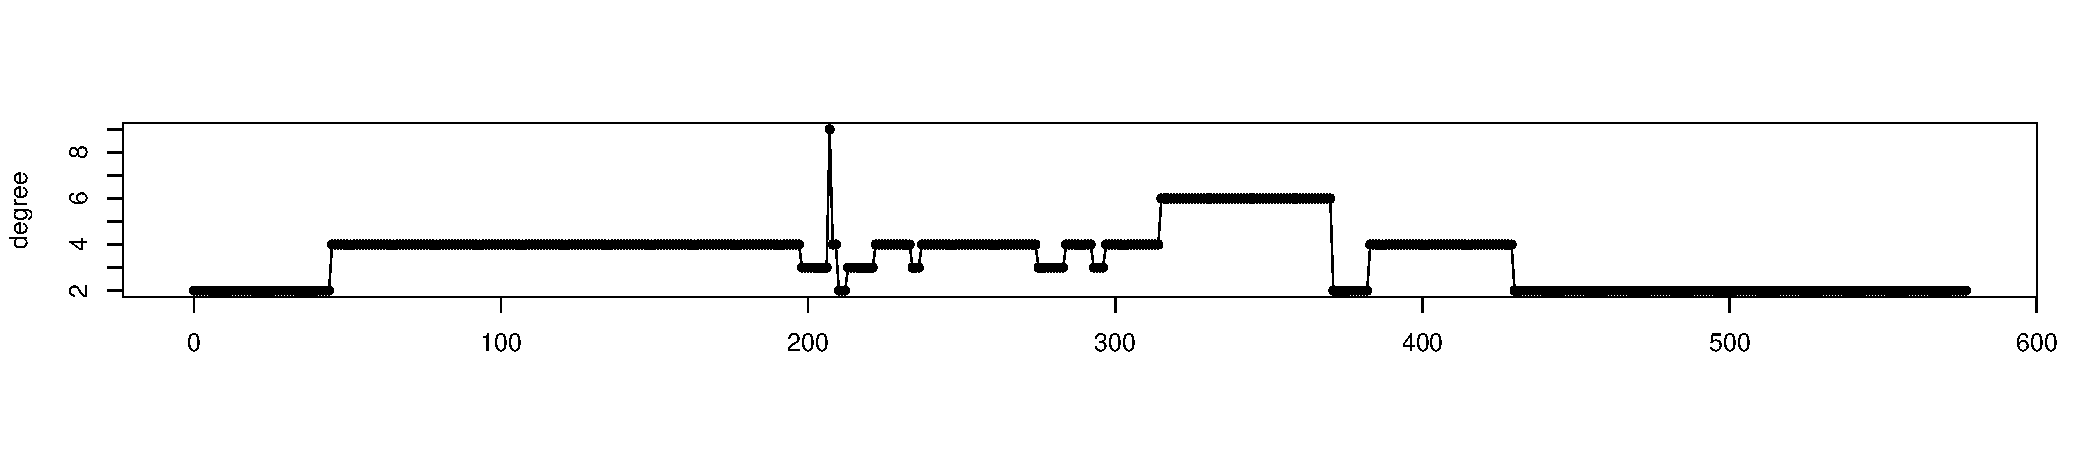
\includegraphics[width=\linewidth,trim=+.225cm 0 +.425cm +2cm]{fig/metrics/chr4_HTT_chm13_degree_w1_bed.pdf}  
		\label{fig:metrics-degree}
	\end{subfigure}
%	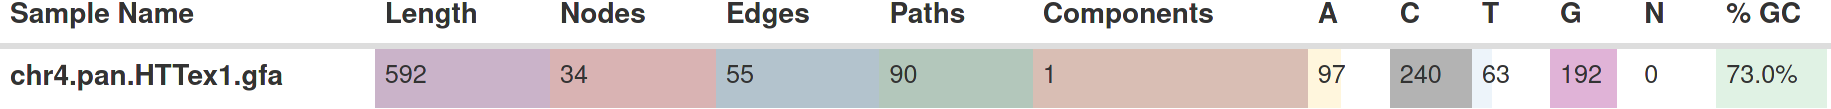
\includegraphics[width=\linewidth]{fig/metrics/chr4.pan.HTTex1.gfa.multiqc_odgi_stats.png}
	\caption{Visualizing the (\textit{C4 locus}) from a human pangenome graph of 90 haplotypes: \textbf{(a)} standard mode: explain the bio stuff. \textbf{(b)} odgi viz's color by path position: explain the bio stuff XXX. \textbf{(c)} odgi viz's color by strandness: explain the bio stuff XXX. `textbf{(d)}  odgi viz's color by coverage: explain the bio stuff XXX.}
	\label{fig:odgi_viz}
\end{figure*}
